\subsection{What is a Programming Language?}
\begin{frame}{\textbf{What is a Programming Language?}}
    A Programming language is ...
    \begin{itemize}[<+->]
        \item used to tell a computer what to do
        \item usually artificial
    \end{itemize}
\end{frame}

\subsection{Grouping Languages by Domain}
\begin{frame}{\textbf{Grouping Languages by domain}}
    Languages are usually grouped into two categories when based on their specificity
    \begin{itemize}[<+->]
        \item DSLs, small,  targeted at specific problems. Internal/embedded vs external 
        \item GPLs, large, many uses.
    \end{itemize}
\end{frame}
\subsection*{Grouping Languages by Domain}
\begin{frame}{\textbf{Grouping Languages by domain}}
    \begin{figure}[!h]
        \centering
        \begin{tabular}{|c|c|c|c|}
            \hline
            \textbf{Characteristic} &\textbf{DSL } &\textbf{GPL}\\
            \hline
            \textbf{Domain} & Small and well-defined domain & Generality, many use cases\\
            \hline
            \textbf{Size} &Small ASTs & Large ASTs, often user extensible\\
            \hline
            \textbf{Lifespan} &As long as their domain &years to decades\\
            \hline
            \textbf{Extensibility} &Usually not extendible & Extendable\\
            \hline
        \end{tabular}%
        \caption{Comparison between GPLs and DSLs}
    \end{figure}%
\end{frame}


\subsection{Syntax and Semantics}
\begin{frame}{\textbf{Syntax and Semantics}}
    \begin{block}{Definition}
        All languages consist of two parts
        \begin{itemize}[<+->]
            \item \textbf{Syntax} - Defines shape
            \item \textbf{Semantics} - Defines meaning
        \end{itemize}
    \end{block}
    \Large
    Syntax is defined by a grammar.\\
    Grammar is not covered in this course :)
\end{frame}


\subsection{Meta Programming}
\begin{frame}{\textbf{Meta Programming}}
    A metaprogram is a program that works on \textit{other} programs.\\
    Compilers and Interpreters are examples of metaprograms
    \begin{block}{Definition}
        \begin{itemize}
            \item \textbf{Object Language} - Langage that gets compiled/interpreter
            \item \textbf{Meta Language} - Language used to implement the compiler/interpreter
        \end{itemize}
    \end{block}
\end{frame}

\subsection{Sum of Products}
\begin{frame}[fragile]{\textbf{Sum of Products}}
    \begin{figure}
        \centering
        \begin{minipage}{.5\textwidth}
            \begin{lstlisting}[language=Haskell]
    data SomeType = A Bool Bool Bool
                    | B Bool
                    | C
            \end{lstlisting}
        \end{minipage} 
    \end{figure}
    
    \begin{examples}
        \begin{equation*}
            \underbrace{(\text{Bool} \times \text{Bool} \times \text{Bool})}_{A} + \underbrace{\text{Bool}}_{B} + \underbrace{1}_{C}
        \end{equation*}
        \texttt{Bool} is either \texttt{True} or \texttt{False}.\\
        The total number of values of type SomeType is $8 + 2 + 1 = 11$.
    \end{examples}
\end{frame}

\subsection*{Sum of Products}
\begin{frame}[fragile]{\textbf{Sum of Products}}
    \begin{figure}
        \centering
        \begin{minipage}{\textwidth}
            \centering
            \begin{lstlisting}[language=Java]
    interface SomeType {}
    class A implements SomeType {
        boolean a;
        boolean b;
        boolean c ;
    }
    class B implements SomeType {
        boolean a;
    }
    class C implements SomeType {
    }
            \end{lstlisting}
        \end{minipage}
        \caption{Sum of Products in Java}
    \end{figure}
\end{frame}

\subsection*{Q\&A}
\begin{frame}{Questions?}
    \begin{figure}
        \centering
        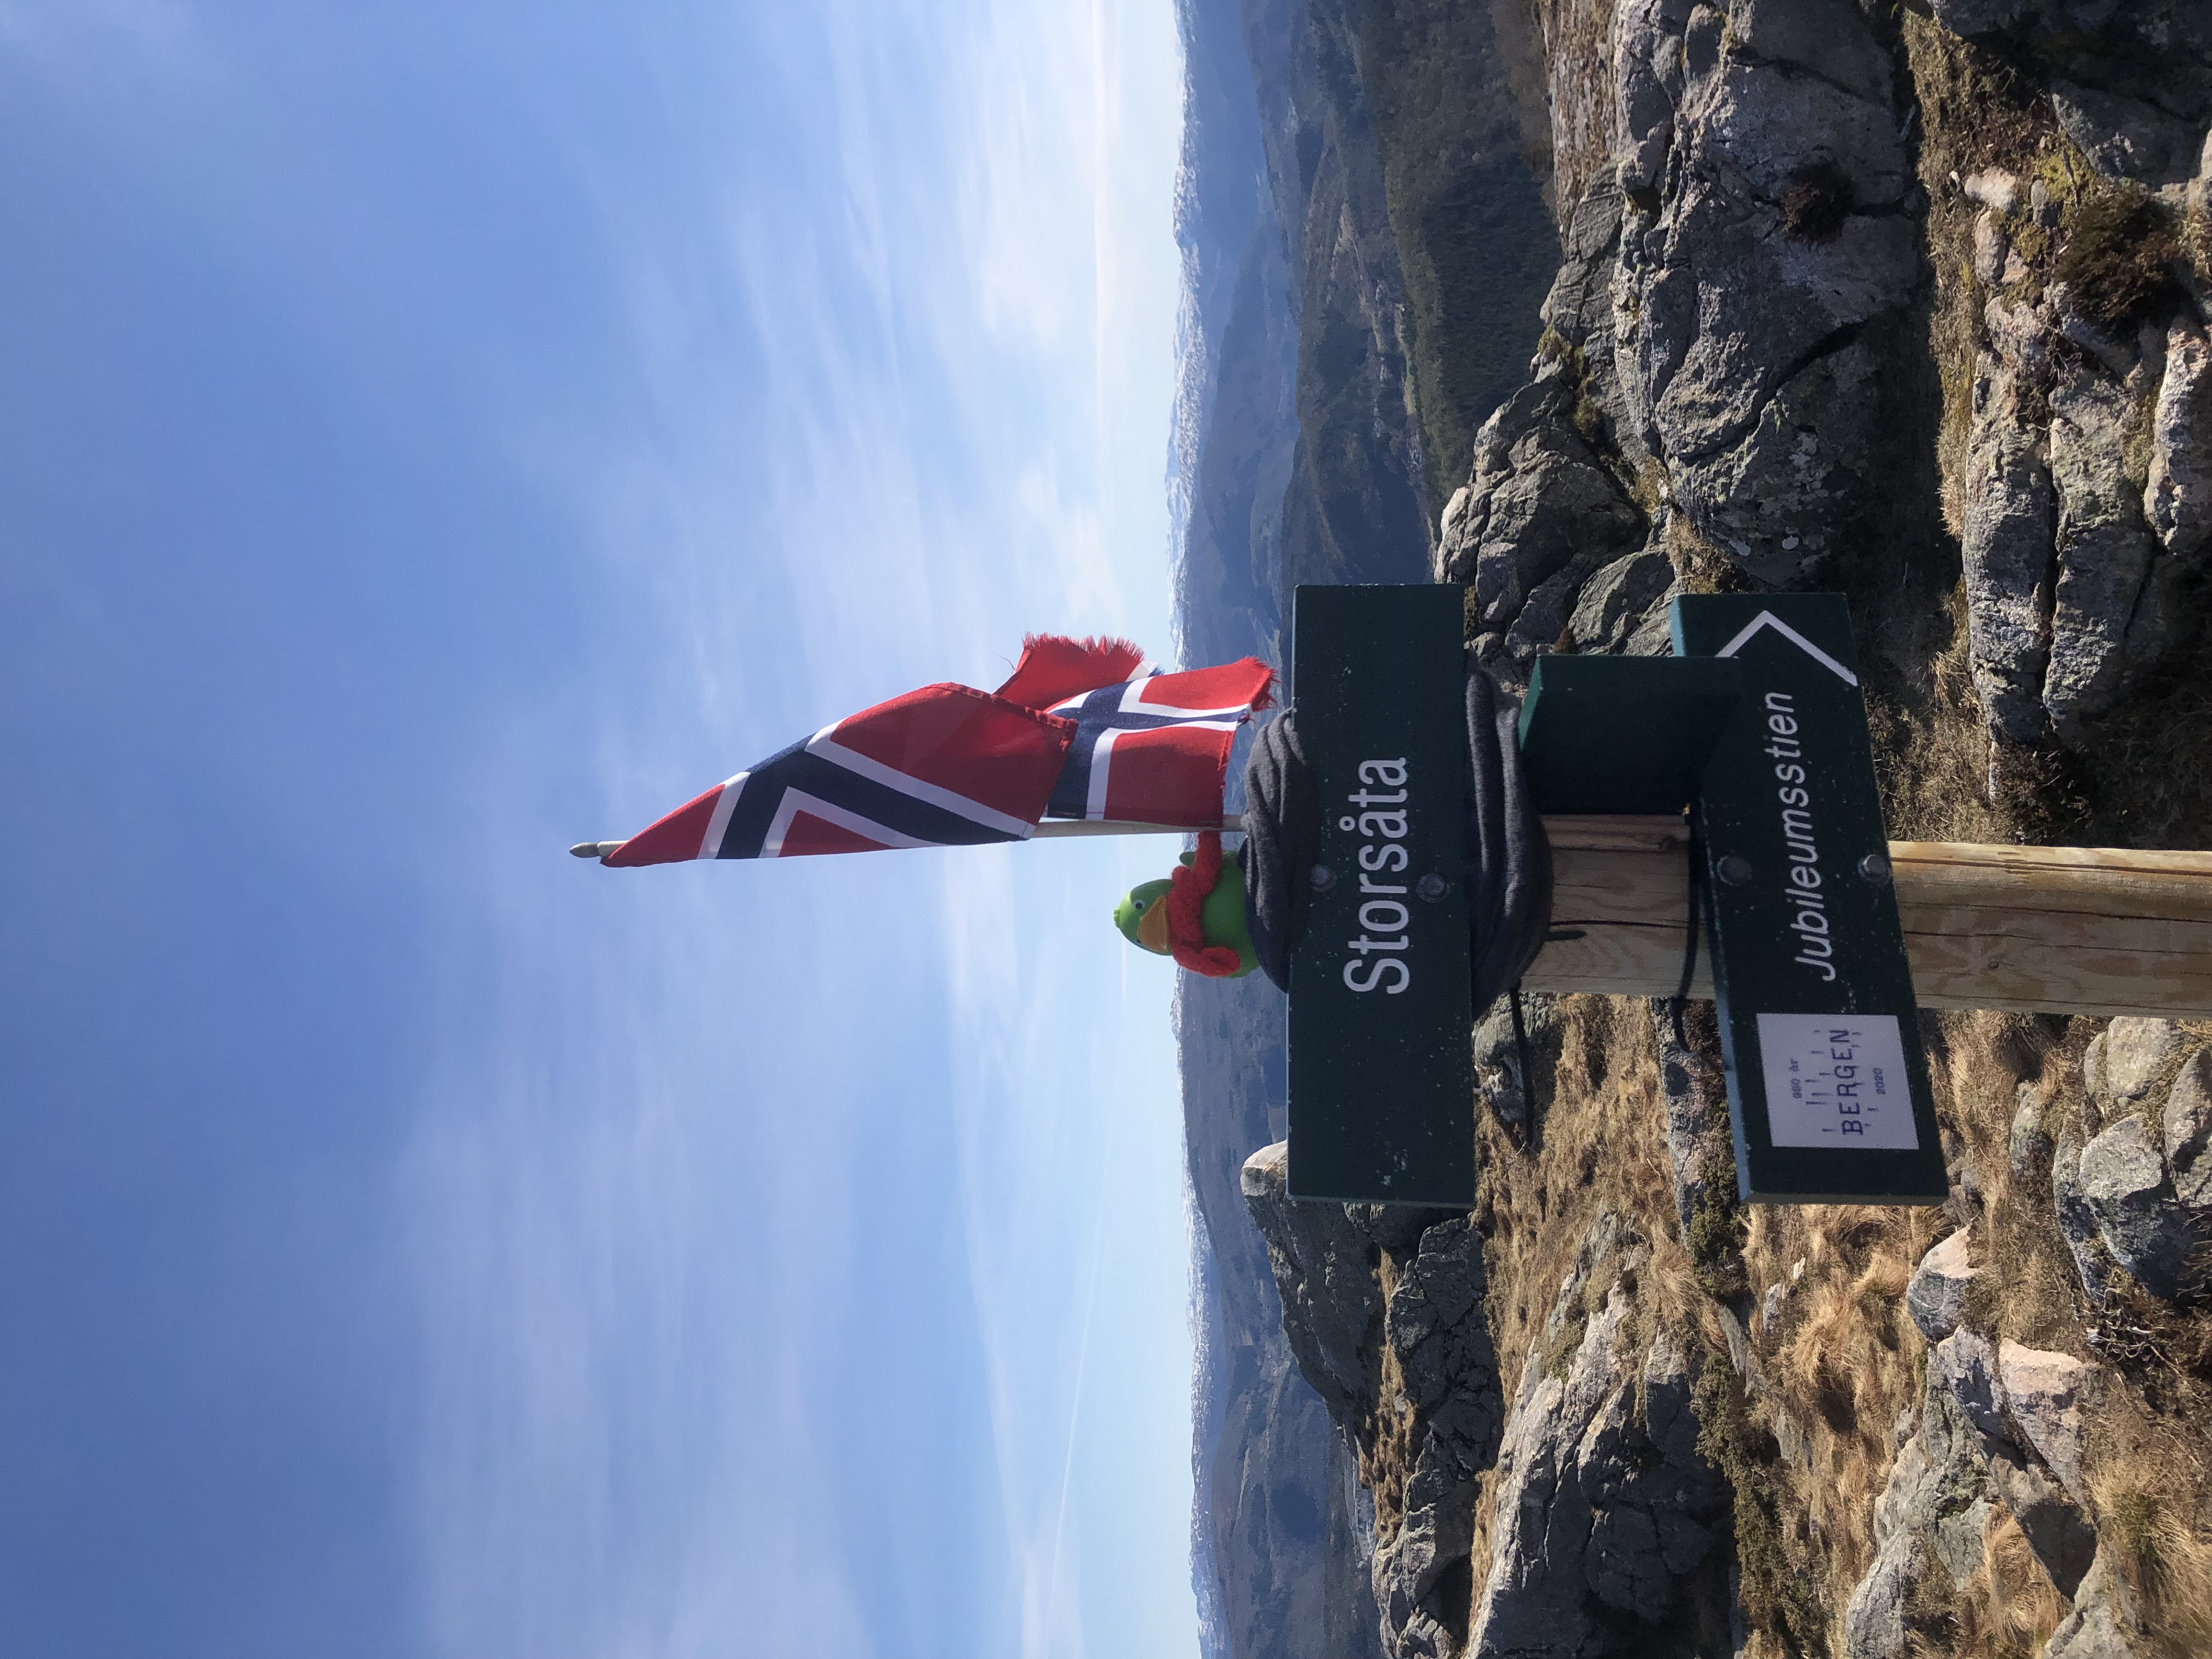
\includegraphics[height = 4.9cm]{guillaume2.jpg}
    \end{figure}
\end{frame}
